We conduct extensive experiments on various aspects of \emph{Altsplit}. We
demonstrate its scalability in Section~\ref{sec:altsplit_scalability} and
show that it is applicable in different machines by providing results on
two HPC clusters in Section~\ref{sec:altsplit_vers}. In Section~\ref{sec:altsplit_trace}
we visualize the \emph{Altsplit} and the \emph{baseline} approach to get more
insights.

\subsection{Parallelism Scalability}
\label{sec:altsplit_scalability}
We run \emph{Altsplit} and \emph{baseline} side-by-side on the x86 clusters
up to 16 nodes (640 MPI threads). We use a total of 4 configurations of MLP networks: 
\begin{itemize}
   \item 16,000-neuron-per-layer, 3-layer, batch size of 512, denoted as 16000.3.512
   \item 16,000-neuron-per-layer, 3-layer, batch size of 1024, denoted as 16000.3.1024
   \item 16,000-neuron-per-layer, 5-layer, batch size of 512, denoted as 16000.5.512
   \item 16,000-neuron-per-layer, 5-layer, batch size of 1024, denoted as 16000.5.1024
\end{itemize}
We measure the elapse time of runs of 50 batches (51 batches but excluding the result from
the first batch to minimize system noises). We execute them on the dataset from 
Cifar-10~\cite{cifar10}. We use 40 MPI threads per node which are mapped to 40 distinct
physical cores. Hence, the measurements are taken in a stride of 40 MPI threads.

Figure~\ref{fig:altsplit_16k_mn4} shows the results in 4 plots. Each plot 
depicts the performance of \emph{Altsplit} against \emph{baseline} in terms of 
elapse time normalized with regard to \emph{baseline} with varied number of MPI 
threads, from 80 MPI threads (2 nodes) all the way up to 640 MPI threads (16 nodes).

We can see from the top left plot (80 MPI threads) that \emph{Altsplit} goes slower than
\emph{baseline}. Nevertheless, starting from 160 MPI threads (top right) and beyond 
\emph{Altsplit} begins to gain track and consistently outperforms \emph{baseline}. 
More specifically, \emph{Altsplit} runs 18.3\%, 39.32\% and 66.11\% faster than their 
respective \emph{baseline} in average.

\begin{figure}[H]
    \centerline{
        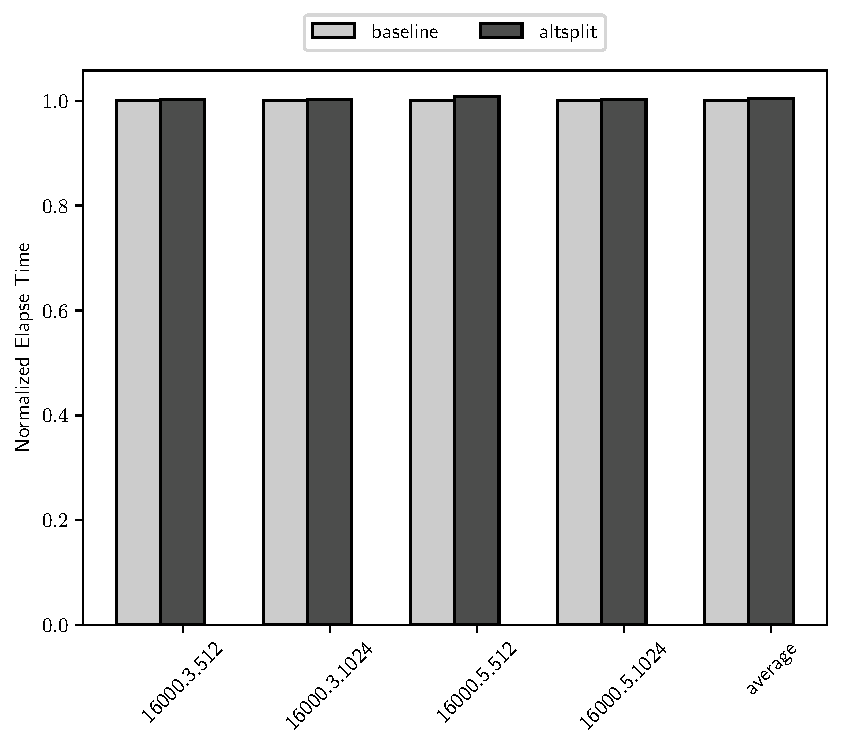
\includegraphics[scale=0.60]{altsplit/figs/mn4/16000_avgs_80.pdf}
        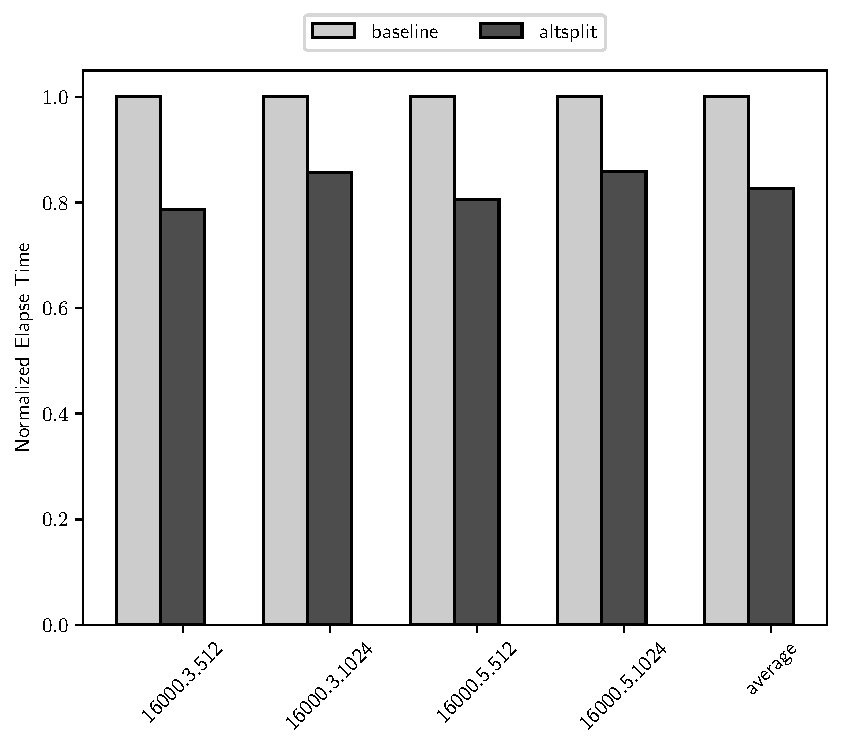
\includegraphics[scale=0.60]{altsplit/figs/mn4/16000_avgs_160.pdf}
    }
    \centerline{
        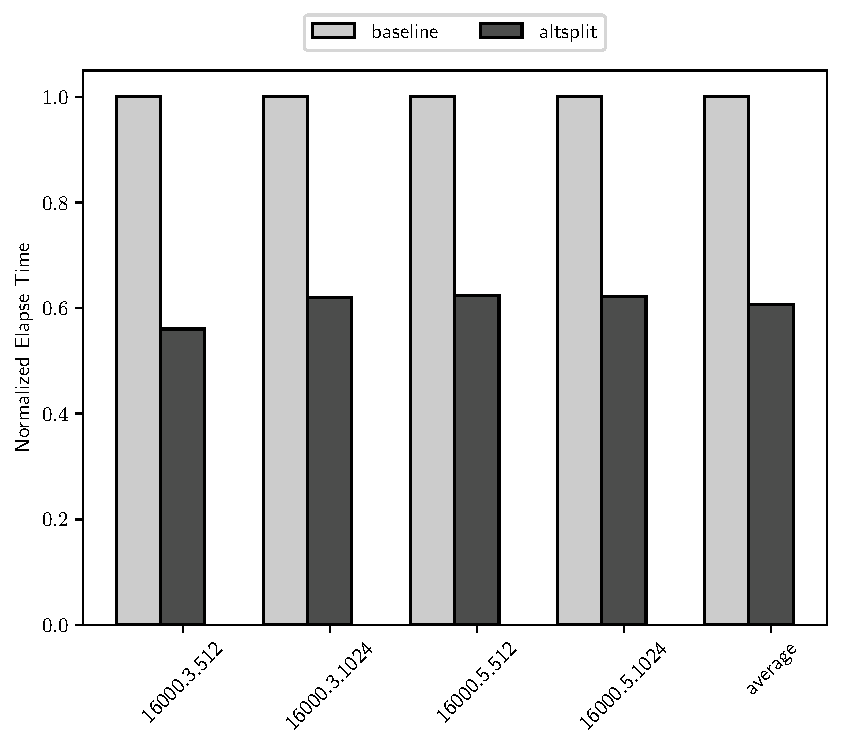
\includegraphics[scale=0.60]{altsplit/figs/mn4/16000_avgs_320.pdf}
        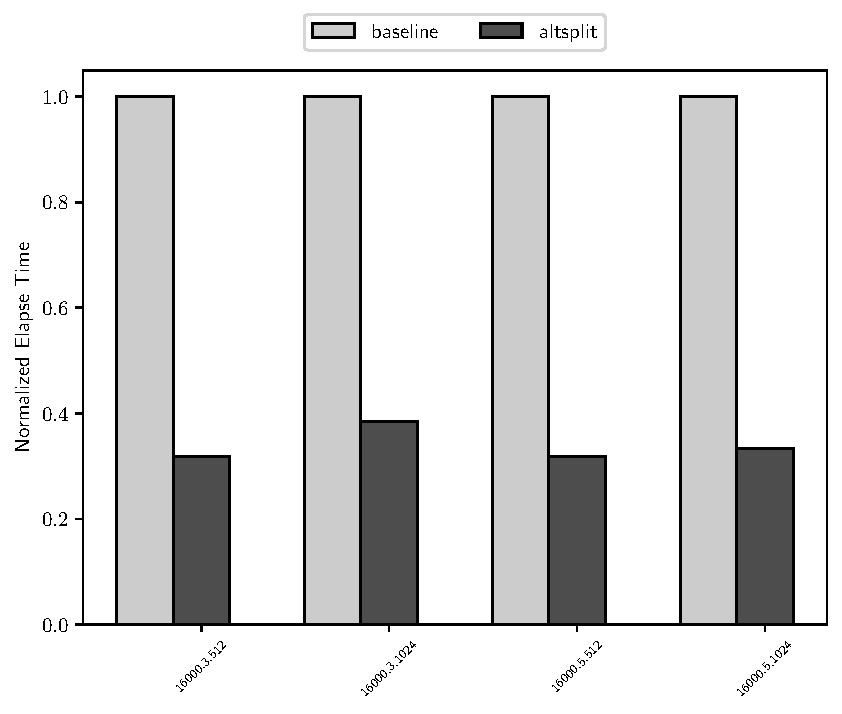
\includegraphics[scale=0.60]{altsplit/figs/mn4/16000_avgs_640.pdf}
    }
    \caption{Performance improvements of 16k neurons on x86. Top left: 80 MPI 
    processes, Top right: 160 MPI processes, Bottom left: 320 MPI processes, 
    Bottom right: 640 MPI processes}
    \label{fig:altsplit_16k_mn4}
\end{figure}

\subsection{Network Versatility}
\label{sec:altsplit_vers}
We launch a more extensive set of experiment that covers more network
configurations. We use two neurons-per-layer numbers: 16k and 32k, two
layers: 3 and 5 along with two batch sizes: 512 and 1024 on both machines. We
find out that \emph{Altsplit} achieves the greatest performance gain on 640
MPI threads (16 nodes on both machines). Table~\ref{table:altsplit_network}
illustrates the results we obtain from of all the configurations.

We observe that \emph{Altsplit} with 16k neurons-per-layer outperforms
\emph{baseline} over 66.12\% and 55.47\% on x86 and POWER9 respectively
whereas with 32k neurons-per-layer the figures are 41.10\% and 32.64\%
respectively. A low neuron-per-layer count attributes to a better performance
with an average gain in average of 25.02\% and 24.51\% respectively on x86
and POWER9. Since we are effectively trading communication with additional
computation with the \emph{Altsplit} approach. In general \emph{Altsplit} also
performs better under smaller batch sizes. This indicates that there is a sweet 
spot where the benefit of reducing the communication is maximized.

\begin{table}[H]
\caption{Performance improvements over the \emph{baseline} on 640 MPI threads}
    \centering
    \begin{tabular}{|P{2.5cm}|P{2.5cm}|P{2.5cm}|P{2.5cm}|P{2.5cm}|}
    \hline
    \multicolumn{3}{|c}{Parameters} & \multicolumn{2}{|c|}{Machine} \\ \hline
    Neurons & Layers & BS & \textbf{x86}  & \textbf{POWER9}  \\ \hline
    \multirow{4}{*}{16k} & \multirow{2}{*}{3} & 512 & 68.12\%& 58.65\%
        \\ \cline{3-5}
     & & 1024 & 61.47\% & 56.12\%
        \\ \cline{2-5}
     & \multirow{2}{*}{5} & 512 & 68.21\%& 58.43\%
        \\ \cline{3-5}
     & & 1024 & 66.68\%& 55.47\%
        \\ \hline 
    \multicolumn{3}{|c|}{Average} & 66.12\% & 57.16\% \\ \hline
     \multirow{4}{*}{32k} & \multirow{2}{*}{3} & 512 & 45.28\% & 32.75\%
        \\ \cline{3-5}
     & & 1024 & 37.69\% & 31.58\%
        \\ \cline{2-5}
     & \multirow{2}{*}{5} & 512 & 43.87\% & 34.37\%
        \\ \cline{3-5}
     & & 1024 & 37.58\%& 31.91\%
        \\ \hline 
    \multicolumn{3}{|c|}{Average} & 41.10\% & 32.65\% \\ \hline
\end{tabular}
\label{table:altsplit_network}
\end{table}


\subsection{Traces}
\label{sec:altsplit_trace}
We run both the \emph{Altsplit} and \emph{baseline} on the x86 cluster with
80 MPI threads and generate running traces. Figure~\ref{fig:altsplit_traces}
illustrates a run with 10 batches (9 are actually shown to exclude the system
noises introduced by the first batch). The x-axis represents the elapse time
whereas each row from the y-axis is the chronological activity from one of
the 80 MPI threads. MPI calls are displayed as the short burst of colored
lines in the traces and the blank areas represents computation or other
system activities. Their length are proportional to the total elapse time.
Two types of MPI all-to-all communication involved in the \emph{baseline}
implementation, namely, MPI\_Allreduce and MPI\_Allgather which corresponds
with the trace on the top. Those marked with red are calls from
MPI\_Allgather while the pink ones are calls from MPI\_Allreduce. The
duration of the trace of the \emph{Altsplit} is the same as in the
\emph{baseline}. One batch in the trace of the \emph{baseline} is marked with
two consecutive MPI\_Allgather (red) calls followed with two MPI\_Allreduce
(pink) ones. On the other hand, in the trace of \emph{Altsplit} one batch is
marked with two MPI\_Allreduce calls with a blank area sparsely dotted with small
bursts of MPI calls. The dark blue activities displayed at the end of both
traces are MPI\_Finalize calls to mark the end of the MPI execution.

We can see that despite the similar duration of MPI\_Allreduce calls on both
approaches and the fact that it takes a longer time for the \emph{Altsplit} to 
commence the subsequent batch, the additional MPI\_Allgather incur a significant 
slow down compared to the blank area in-between the successive MPI\_Allreduce 
calls from the \emph{Altsplit} approach.

\begin{figure}[H]
    \centerline{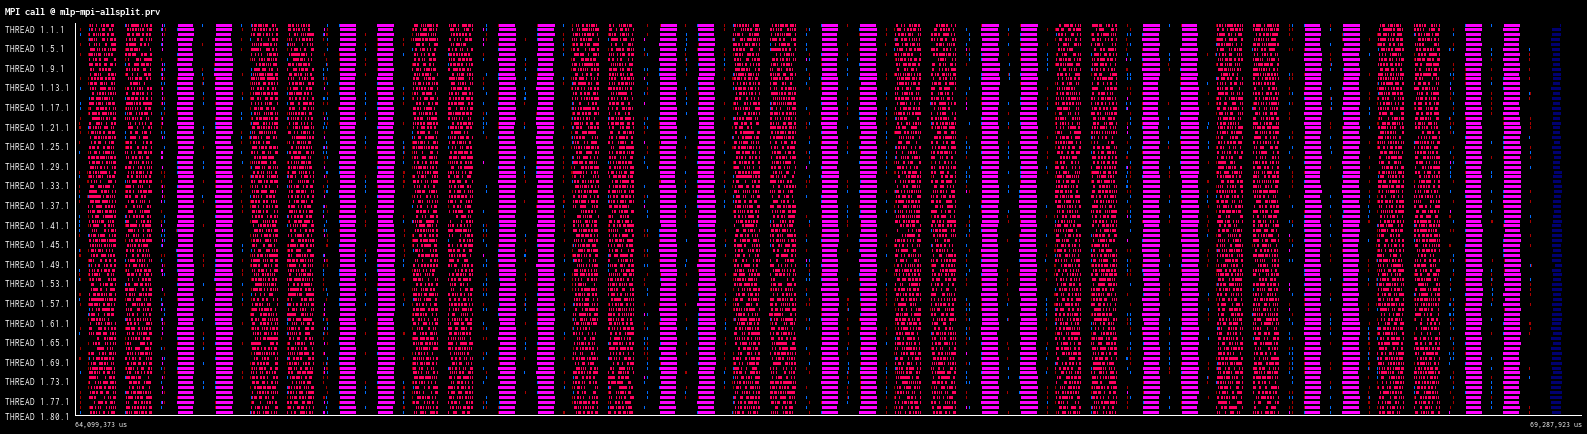
\includegraphics[scale=0.30]{altsplit/figs/baseline_trace.png}}
    \centerline{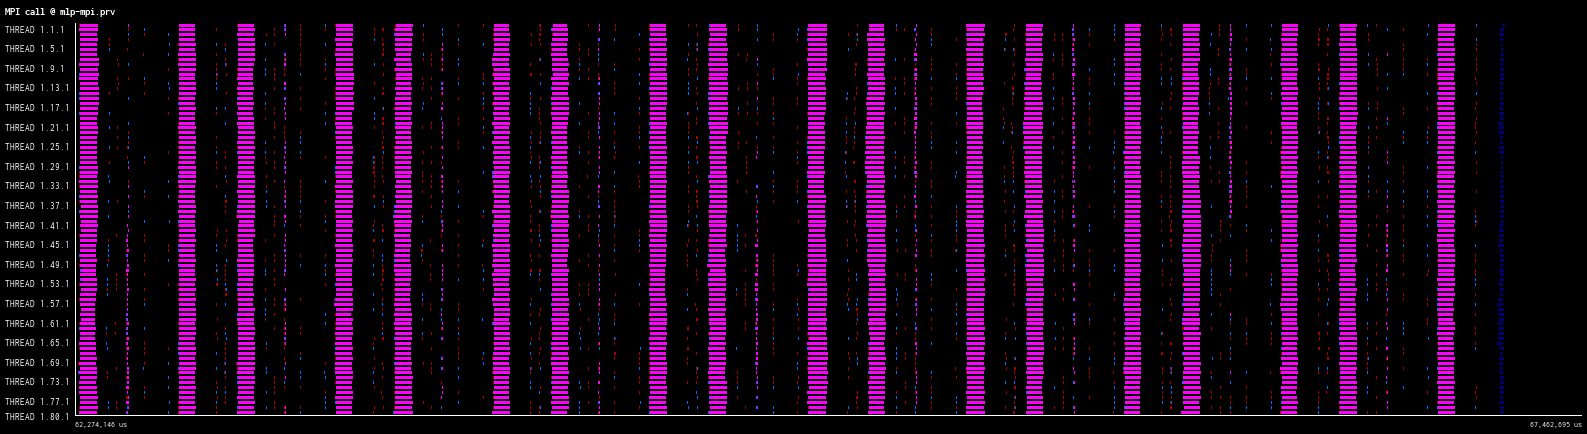
\includegraphics[scale=0.30]{altsplit/figs/altsplit_trace.png}}
    \caption{Traces on 80 MPI processes 9 batches. Top: \emph{baseline} approach Bottom: \emph{altsplit} approach}
    \label{fig:altsplit_traces}
\end{figure}
